% Options for packages loaded elsewhere
\PassOptionsToPackage{unicode}{hyperref}
\PassOptionsToPackage{hyphens}{url}
\PassOptionsToPackage{dvipsnames,svgnames,x11names}{xcolor}
%
\documentclass[
  letterpaper,
  DIV=11,
  numbers=noendperiod]{scrartcl}

\usepackage{amsmath,amssymb}
\usepackage{iftex}
\ifPDFTeX
  \usepackage[T1]{fontenc}
  \usepackage[utf8]{inputenc}
  \usepackage{textcomp} % provide euro and other symbols
\else % if luatex or xetex
  \usepackage{unicode-math}
  \defaultfontfeatures{Scale=MatchLowercase}
  \defaultfontfeatures[\rmfamily]{Ligatures=TeX,Scale=1}
\fi
\usepackage{lmodern}
\ifPDFTeX\else  
    % xetex/luatex font selection
\fi
% Use upquote if available, for straight quotes in verbatim environments
\IfFileExists{upquote.sty}{\usepackage{upquote}}{}
\IfFileExists{microtype.sty}{% use microtype if available
  \usepackage[]{microtype}
  \UseMicrotypeSet[protrusion]{basicmath} % disable protrusion for tt fonts
}{}
\makeatletter
\@ifundefined{KOMAClassName}{% if non-KOMA class
  \IfFileExists{parskip.sty}{%
    \usepackage{parskip}
  }{% else
    \setlength{\parindent}{0pt}
    \setlength{\parskip}{6pt plus 2pt minus 1pt}}
}{% if KOMA class
  \KOMAoptions{parskip=half}}
\makeatother
\usepackage{xcolor}
\setlength{\emergencystretch}{3em} % prevent overfull lines
\setcounter{secnumdepth}{-\maxdimen} % remove section numbering
% Make \paragraph and \subparagraph free-standing
\makeatletter
\ifx\paragraph\undefined\else
  \let\oldparagraph\paragraph
  \renewcommand{\paragraph}{
    \@ifstar
      \xxxParagraphStar
      \xxxParagraphNoStar
  }
  \newcommand{\xxxParagraphStar}[1]{\oldparagraph*{#1}\mbox{}}
  \newcommand{\xxxParagraphNoStar}[1]{\oldparagraph{#1}\mbox{}}
\fi
\ifx\subparagraph\undefined\else
  \let\oldsubparagraph\subparagraph
  \renewcommand{\subparagraph}{
    \@ifstar
      \xxxSubParagraphStar
      \xxxSubParagraphNoStar
  }
  \newcommand{\xxxSubParagraphStar}[1]{\oldsubparagraph*{#1}\mbox{}}
  \newcommand{\xxxSubParagraphNoStar}[1]{\oldsubparagraph{#1}\mbox{}}
\fi
\makeatother

\usepackage{color}
\usepackage{fancyvrb}
\newcommand{\VerbBar}{|}
\newcommand{\VERB}{\Verb[commandchars=\\\{\}]}
\DefineVerbatimEnvironment{Highlighting}{Verbatim}{commandchars=\\\{\}}
% Add ',fontsize=\small' for more characters per line
\usepackage{framed}
\definecolor{shadecolor}{RGB}{241,243,245}
\newenvironment{Shaded}{\begin{snugshade}}{\end{snugshade}}
\newcommand{\AlertTok}[1]{\textcolor[rgb]{0.68,0.00,0.00}{#1}}
\newcommand{\AnnotationTok}[1]{\textcolor[rgb]{0.37,0.37,0.37}{#1}}
\newcommand{\AttributeTok}[1]{\textcolor[rgb]{0.40,0.45,0.13}{#1}}
\newcommand{\BaseNTok}[1]{\textcolor[rgb]{0.68,0.00,0.00}{#1}}
\newcommand{\BuiltInTok}[1]{\textcolor[rgb]{0.00,0.23,0.31}{#1}}
\newcommand{\CharTok}[1]{\textcolor[rgb]{0.13,0.47,0.30}{#1}}
\newcommand{\CommentTok}[1]{\textcolor[rgb]{0.37,0.37,0.37}{#1}}
\newcommand{\CommentVarTok}[1]{\textcolor[rgb]{0.37,0.37,0.37}{\textit{#1}}}
\newcommand{\ConstantTok}[1]{\textcolor[rgb]{0.56,0.35,0.01}{#1}}
\newcommand{\ControlFlowTok}[1]{\textcolor[rgb]{0.00,0.23,0.31}{\textbf{#1}}}
\newcommand{\DataTypeTok}[1]{\textcolor[rgb]{0.68,0.00,0.00}{#1}}
\newcommand{\DecValTok}[1]{\textcolor[rgb]{0.68,0.00,0.00}{#1}}
\newcommand{\DocumentationTok}[1]{\textcolor[rgb]{0.37,0.37,0.37}{\textit{#1}}}
\newcommand{\ErrorTok}[1]{\textcolor[rgb]{0.68,0.00,0.00}{#1}}
\newcommand{\ExtensionTok}[1]{\textcolor[rgb]{0.00,0.23,0.31}{#1}}
\newcommand{\FloatTok}[1]{\textcolor[rgb]{0.68,0.00,0.00}{#1}}
\newcommand{\FunctionTok}[1]{\textcolor[rgb]{0.28,0.35,0.67}{#1}}
\newcommand{\ImportTok}[1]{\textcolor[rgb]{0.00,0.46,0.62}{#1}}
\newcommand{\InformationTok}[1]{\textcolor[rgb]{0.37,0.37,0.37}{#1}}
\newcommand{\KeywordTok}[1]{\textcolor[rgb]{0.00,0.23,0.31}{\textbf{#1}}}
\newcommand{\NormalTok}[1]{\textcolor[rgb]{0.00,0.23,0.31}{#1}}
\newcommand{\OperatorTok}[1]{\textcolor[rgb]{0.37,0.37,0.37}{#1}}
\newcommand{\OtherTok}[1]{\textcolor[rgb]{0.00,0.23,0.31}{#1}}
\newcommand{\PreprocessorTok}[1]{\textcolor[rgb]{0.68,0.00,0.00}{#1}}
\newcommand{\RegionMarkerTok}[1]{\textcolor[rgb]{0.00,0.23,0.31}{#1}}
\newcommand{\SpecialCharTok}[1]{\textcolor[rgb]{0.37,0.37,0.37}{#1}}
\newcommand{\SpecialStringTok}[1]{\textcolor[rgb]{0.13,0.47,0.30}{#1}}
\newcommand{\StringTok}[1]{\textcolor[rgb]{0.13,0.47,0.30}{#1}}
\newcommand{\VariableTok}[1]{\textcolor[rgb]{0.07,0.07,0.07}{#1}}
\newcommand{\VerbatimStringTok}[1]{\textcolor[rgb]{0.13,0.47,0.30}{#1}}
\newcommand{\WarningTok}[1]{\textcolor[rgb]{0.37,0.37,0.37}{\textit{#1}}}

\providecommand{\tightlist}{%
  \setlength{\itemsep}{0pt}\setlength{\parskip}{0pt}}\usepackage{longtable,booktabs,array}
\usepackage{calc} % for calculating minipage widths
% Correct order of tables after \paragraph or \subparagraph
\usepackage{etoolbox}
\makeatletter
\patchcmd\longtable{\par}{\if@noskipsec\mbox{}\fi\par}{}{}
\makeatother
% Allow footnotes in longtable head/foot
\IfFileExists{footnotehyper.sty}{\usepackage{footnotehyper}}{\usepackage{footnote}}
\makesavenoteenv{longtable}
\usepackage{graphicx}
\makeatletter
\def\maxwidth{\ifdim\Gin@nat@width>\linewidth\linewidth\else\Gin@nat@width\fi}
\def\maxheight{\ifdim\Gin@nat@height>\textheight\textheight\else\Gin@nat@height\fi}
\makeatother
% Scale images if necessary, so that they will not overflow the page
% margins by default, and it is still possible to overwrite the defaults
% using explicit options in \includegraphics[width, height, ...]{}
\setkeys{Gin}{width=\maxwidth,height=\maxheight,keepaspectratio}
% Set default figure placement to htbp
\makeatletter
\def\fps@figure{htbp}
\makeatother

\usepackage{fvextra}
\DefineVerbatimEnvironment{Highlighting}{Verbatim}{breaklines,commandchars=\\\{\}}
\DefineVerbatimEnvironment{OutputCode}{Verbatim}{breaklines,commandchars=\\\{\}}
\KOMAoption{captions}{tableheading}
\makeatletter
\@ifpackageloaded{caption}{}{\usepackage{caption}}
\AtBeginDocument{%
\ifdefined\contentsname
  \renewcommand*\contentsname{Table of contents}
\else
  \newcommand\contentsname{Table of contents}
\fi
\ifdefined\listfigurename
  \renewcommand*\listfigurename{List of Figures}
\else
  \newcommand\listfigurename{List of Figures}
\fi
\ifdefined\listtablename
  \renewcommand*\listtablename{List of Tables}
\else
  \newcommand\listtablename{List of Tables}
\fi
\ifdefined\figurename
  \renewcommand*\figurename{Figure}
\else
  \newcommand\figurename{Figure}
\fi
\ifdefined\tablename
  \renewcommand*\tablename{Table}
\else
  \newcommand\tablename{Table}
\fi
}
\@ifpackageloaded{float}{}{\usepackage{float}}
\floatstyle{ruled}
\@ifundefined{c@chapter}{\newfloat{codelisting}{h}{lop}}{\newfloat{codelisting}{h}{lop}[chapter]}
\floatname{codelisting}{Listing}
\newcommand*\listoflistings{\listof{codelisting}{List of Listings}}
\makeatother
\makeatletter
\makeatother
\makeatletter
\@ifpackageloaded{caption}{}{\usepackage{caption}}
\@ifpackageloaded{subcaption}{}{\usepackage{subcaption}}
\makeatother

\ifLuaTeX
  \usepackage{selnolig}  % disable illegal ligatures
\fi
\usepackage{bookmark}

\IfFileExists{xurl.sty}{\usepackage{xurl}}{} % add URL line breaks if available
\urlstyle{same} % disable monospaced font for URLs
\hypersetup{
  pdftitle={BST 270: Individual Project},
  pdfauthor={Keyao Zhan},
  colorlinks=true,
  linkcolor={blue},
  filecolor={Maroon},
  citecolor={Blue},
  urlcolor={Blue},
  pdfcreator={LaTeX via pandoc}}


\title{BST 270: Individual Project}
\usepackage{etoolbox}
\makeatletter
\providecommand{\subtitle}[1]{% add subtitle to \maketitle
  \apptocmd{\@title}{\par {\large #1 \par}}{}{}
}
\makeatother
\subtitle{Reproducible Data Science: How Americans Like Their Steak
(FiveThirtyEight)}
\author{Keyao Zhan}
\date{}

\begin{document}
\maketitle


\subsection{Introduction}\label{introduction}

The following notebook aims to satisfy the requirements for the
individual project component of BST 270: Reproducible Data Science,
taken Winter 2025.

\paragraph{Motivations and
Reproducibility}\label{motivations-and-reproducibility}

I aim to reproduce the figure and the table from FiveThirtyEight's
\href{https://fivethirtyeight.com/features/how-americans-like-their-steak/}{How
Americans Like Their Steak}. I will utilize the provided dataset based
on a survey testing 550 people about their risk evaluation and steak
preference, located at \texttt{../data/steak-risk-survey.csv}.

\subsection{Setup}\label{setup}

First, we load our required packages and required dataset. We utilize
the \texttt{dplyr}, \texttt{knitr} and \texttt{ggplot2} library to
produce nice figures and tables and process data efficiently.

\begin{verbatim}

Attaching package: 'dplyr'
\end{verbatim}

\begin{verbatim}
The following objects are masked from 'package:stats':

    filter, lag
\end{verbatim}

\begin{verbatim}
The following objects are masked from 'package:base':

    intersect, setdiff, setequal, union
\end{verbatim}

Here we remove the first two rows which are of no information.

\begin{Shaded}
\begin{Highlighting}[]
\CommentTok{\# Remove first two invalid rows}
\NormalTok{steak\_data }\OtherTok{\textless{}{-}} \FunctionTok{read.csv}\NormalTok{(}\StringTok{"../data/steak{-}risk{-}survey.csv"}\NormalTok{,}\AttributeTok{header =}\NormalTok{ T)}
\NormalTok{steak\_data }\OtherTok{=}\NormalTok{ steak\_data[}\SpecialCharTok{{-}}\FunctionTok{c}\NormalTok{(}\DecValTok{1}\NormalTok{,}\DecValTok{2}\NormalTok{),]}
\end{Highlighting}
\end{Shaded}

The original dataset has too long names and some irrelevant variables,
so we extract a new dataset that is useful for our analysis.

\begin{Shaded}
\begin{Highlighting}[]
\CommentTok{\# Filter and rename the dataset}
\NormalTok{steak\_lottery\_data }\OtherTok{=} \FunctionTok{data.frame}\NormalTok{(}\AttributeTok{lottery =}\NormalTok{ steak\_data}\SpecialCharTok{$}\NormalTok{Consider.the.following.hypothetical.situations...br.In.Lottery.A..you.have.a.}\DecValTok{50}\NormalTok{..chance.of.success..with.a.payout.of..}\DecValTok{100}\NormalTok{...br.In.Lottery.B..you.have.a.}\DecValTok{90}\NormalTok{..chance.of.success..with.a.payout.of..}\DecValTok{20}\NormalTok{...br..br.Assuming.you.have..}\FloatTok{10.}\NormalTok{to.bet..would.you.play.Lottery.A.or.Lottery.B., }\AttributeTok{eat\_steak =}\NormalTok{ steak\_data}\SpecialCharTok{$}\NormalTok{Do.you.eat.steak.,}\AttributeTok{cook\_steak =}\NormalTok{ steak\_data}\SpecialCharTok{$}\NormalTok{How.do.you.like.your.steak.prepared.)}
\FunctionTok{write.csv}\NormalTok{(steak\_lottery\_data, }\AttributeTok{file =} \StringTok{"../data/steak\_lottery\_data.csv"}\NormalTok{)}
\FunctionTok{head}\NormalTok{(steak\_lottery\_data)}
\end{Highlighting}
\end{Shaded}

\begin{verbatim}
    lottery eat_steak  cook_steak
1 Lottery A       Yes Medium rare
2 Lottery A       Yes        Rare
3 Lottery B       Yes      Medium
4 Lottery B       Yes      Medium
5 Lottery A       Yes Medium rare
6 Lottery A        No            
\end{verbatim}

\subsection{Reproduce the table}\label{reproduce-the-table}

The table in the article shows the pertange of steak preparation
preference of the people who choose a riskier lottery or a safer
lottery.

First we need to remove all the NA (or empty values) in lottery
variable, and focus on people who eats steak:

\begin{Shaded}
\begin{Highlighting}[]
\NormalTok{df1 }\OtherTok{=}\NormalTok{ steak\_lottery\_data }\SpecialCharTok{\%\textgreater{}\%}
  \FunctionTok{filter}\NormalTok{(lottery }\SpecialCharTok{!=} \StringTok{""}\NormalTok{, eat\_steak }\SpecialCharTok{==} \StringTok{"Yes"}\NormalTok{)}
\FunctionTok{dim}\NormalTok{(df1)}
\end{Highlighting}
\end{Shaded}

\begin{verbatim}
[1] 426   3
\end{verbatim}

There are 426 people who answered the lottery question and also eat
steak. Next we reproduce the table:

\begin{Shaded}
\begin{Highlighting}[]
\FunctionTok{kable}\NormalTok{(tb1}\SpecialCharTok{*}\DecValTok{100}\NormalTok{,}\AttributeTok{format =} \StringTok{"pipe"}\NormalTok{,}\AttributeTok{digits =} \DecValTok{1}\NormalTok{)}
\end{Highlighting}
\end{Shaded}

\begin{longtable}[]{@{}lrr@{}}
\toprule\noalign{}
& Riskier lottery & Safer lottery \\
\midrule\noalign{}
\endhead
\bottomrule\noalign{}
\endlastfoot
Well & 7.3 & 9.0 \\
Medium Well & 16.1 & 18.1 \\
Medium & 36.1 & 25.8 \\
Medium rare & 35.6 & 41.2 \\
Rare & 4.9 & 5.9 \\
\end{longtable}

\textbf{Comment:} We nearly recovered the table in the article, with
slight difference.

\subsection{Reproducing Plot}\label{reproducing-plot}

The figure shows the percentage of the steak preparation preference of
all steak eating interviewees. First we filter out all people who eats
steak.

\begin{Shaded}
\begin{Highlighting}[]
\CommentTok{\# Create the counting table}
\NormalTok{df2 }\OtherTok{=}\NormalTok{ steak\_lottery\_data }\SpecialCharTok{\%\textgreater{}\%}
  \FunctionTok{filter}\NormalTok{(eat\_steak }\SpecialCharTok{==} \StringTok{"Yes"}\NormalTok{)}

\NormalTok{prep\_names }\OtherTok{=} \FunctionTok{c}\NormalTok{(}\StringTok{"Rare"}\NormalTok{,}\StringTok{"Medium rare"}\NormalTok{,}\StringTok{"Medium"}\NormalTok{,}\StringTok{"Medium Well"}\NormalTok{,}\StringTok{"Well"}\NormalTok{)}
\NormalTok{df2}\FloatTok{.1} \OtherTok{=} \FunctionTok{data.frame}\NormalTok{(}\FunctionTok{table}\NormalTok{(df2}\SpecialCharTok{$}\NormalTok{cook\_steak)[prep\_names]}\SpecialCharTok{/}\FunctionTok{sum}\NormalTok{(}\FunctionTok{table}\NormalTok{(df2}\SpecialCharTok{$}\NormalTok{cook\_steak))}\SpecialCharTok{*}\DecValTok{100}\NormalTok{)}
\FunctionTok{colnames}\NormalTok{(df2}\FloatTok{.1}\NormalTok{) }\OtherTok{=} \FunctionTok{c}\NormalTok{(}\StringTok{"Cooked"}\NormalTok{,}\StringTok{"Percentage"}\NormalTok{)}
\NormalTok{df2}\FloatTok{.1}
\end{Highlighting}
\end{Shaded}

\begin{verbatim}
       Cooked Percentage
1        Rare   5.348837
2 Medium rare  38.604651
3      Medium  30.697674
4 Medium Well  17.209302
5        Well   8.139535
\end{verbatim}

Next we reproduce the plot in the article:

\begin{Shaded}
\begin{Highlighting}[]
\CommentTok{\# Reproduce the figure}
\NormalTok{gg }\OtherTok{=} \FunctionTok{ggplot}\NormalTok{(df2}\FloatTok{.1}\NormalTok{, }\FunctionTok{aes}\NormalTok{(}\AttributeTok{x =}\NormalTok{ Cooked, }\AttributeTok{y =}\NormalTok{ Percentage)) }\SpecialCharTok{+}
  \FunctionTok{geom\_bar}\NormalTok{(}\AttributeTok{stat =} \StringTok{"identity"}\NormalTok{, }\AttributeTok{fill =} \FunctionTok{rev}\NormalTok{(}\FunctionTok{c}\NormalTok{(}\StringTok{"\#4B2C20"}\NormalTok{, }\StringTok{"\#754637"}\NormalTok{, }\StringTok{"\#AA6546"}\NormalTok{, }\StringTok{"\#C06050"}\NormalTok{, }\StringTok{"\#C93535"}\NormalTok{))) }\SpecialCharTok{+}
  \FunctionTok{coord\_flip}\NormalTok{() }\SpecialCharTok{+}  
  \FunctionTok{geom\_text}\NormalTok{(}\FunctionTok{aes}\NormalTok{(}\AttributeTok{label =} \FunctionTok{paste0}\NormalTok{(}\FunctionTok{round}\NormalTok{(Percentage), }\StringTok{"\%"}\NormalTok{)), }\AttributeTok{hjust =} \SpecialCharTok{{-}}\FloatTok{0.2}\NormalTok{) }\SpecialCharTok{+} 
  \FunctionTok{labs}\NormalTok{(}
    \AttributeTok{title =} \StringTok{"\textquotesingle{}How Do You Like Your Steak Prepared?\textquotesingle{}"}\NormalTok{,}
    \AttributeTok{subtitle =} \FunctionTok{paste}\NormalTok{(}\StringTok{"From a survey of"}\NormalTok{, }\FunctionTok{sum}\NormalTok{(}\FunctionTok{nrow}\NormalTok{(df2)), }\StringTok{"steak{-}eating responses"}\NormalTok{),}
    \AttributeTok{x =} \ConstantTok{NULL}\NormalTok{,}
    \AttributeTok{y =} \ConstantTok{NULL}
\NormalTok{  ) }\SpecialCharTok{+}
  \FunctionTok{theme\_minimal}\NormalTok{() }\SpecialCharTok{+}
  \FunctionTok{theme}\NormalTok{(}
    \AttributeTok{plot.title =} \FunctionTok{element\_text}\NormalTok{(}\AttributeTok{size =} \DecValTok{16}\NormalTok{, }\AttributeTok{face =} \StringTok{"bold"}\NormalTok{),}
    \AttributeTok{plot.subtitle =} \FunctionTok{element\_text}\NormalTok{(}\AttributeTok{size =} \DecValTok{12}\NormalTok{, }\AttributeTok{margin =} \FunctionTok{margin}\NormalTok{(}\AttributeTok{b =} \DecValTok{10}\NormalTok{)),}
    \AttributeTok{axis.text.x =} \FunctionTok{element\_blank}\NormalTok{(),}
    \AttributeTok{axis.text.y =} \FunctionTok{element\_text}\NormalTok{(}\AttributeTok{size =} \DecValTok{12}\NormalTok{),}
    \AttributeTok{axis.ticks =} \FunctionTok{element\_blank}\NormalTok{(),}
    \AttributeTok{aspect.ratio =} \FloatTok{0.25}
\NormalTok{  )}
\NormalTok{gg}
\end{Highlighting}
\end{Shaded}

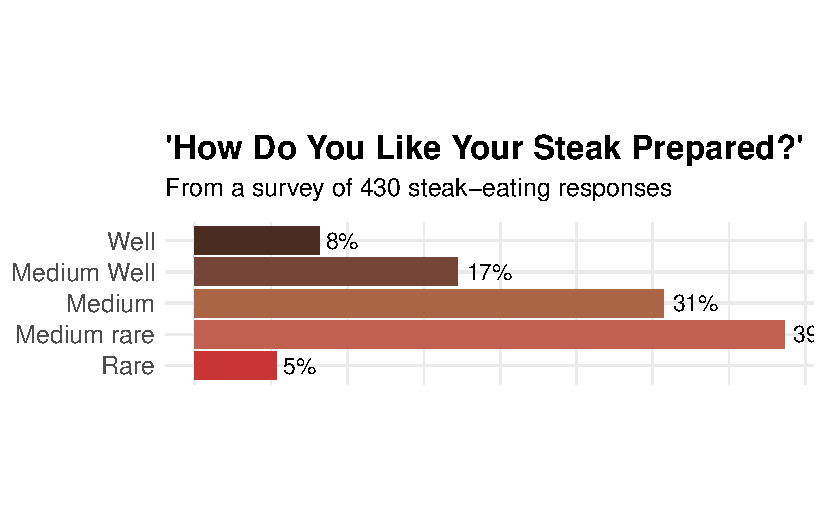
\includegraphics{steak_analysis_files/figure-pdf/unnamed-chunk-7-1.pdf}

\textbf{Comment:} From the plot we see that we nearly reproduced the
figure, only with slight difference in the percentage.

\begin{Shaded}
\begin{Highlighting}[]
\FunctionTok{ggsave}\NormalTok{(}\StringTok{"../fig/steak\_preference.png"}\NormalTok{,}\AttributeTok{plot =}\NormalTok{ gg)}
\end{Highlighting}
\end{Shaded}

\begin{verbatim}
Saving 5.5 x 3.5 in image
\end{verbatim}

\subsection{Reflection on the
reproducibility}\label{reflection-on-the-reproducibility}

This is a quite simple data analysis. The data is publicly available,
and the figure and the table are quite reproducible. I think the only
problem arises in the first two rows I removed. As these two rows are
indeed invalid ones, I guess the author made some mistakes when storing
the data as the csv file.




\end{document}
